\documentclass[1p]{elsarticle_modified}
%\bibliographystyle{elsarticle-num}

%\usepackage[colorlinks]{hyperref}
%\usepackage{abbrmath_seonhwa} %\Abb, \Ascr, \Acal ,\Abf, \Afrak
\usepackage{amsfonts}
\usepackage{amssymb}
\usepackage{amsmath}
\usepackage{amsthm}
\usepackage{scalefnt}
\usepackage{amsbsy}
\usepackage{kotex}
\usepackage{caption}
\usepackage{subfig}
\usepackage{color}
\usepackage{graphicx}
\usepackage{xcolor} %% white, black, red, green, blue, cyan, magenta, yellow
\usepackage{float}
\usepackage{setspace}
\usepackage{hyperref}

\usepackage{tikz}
\usetikzlibrary{arrows}

\usepackage{multirow}
\usepackage{array} % fixed length table
\usepackage{hhline}

%%%%%%%%%%%%%%%%%%%%%
\makeatletter
\renewcommand*\env@matrix[1][\arraystretch]{%
	\edef\arraystretch{#1}%
	\hskip -\arraycolsep
	\let\@ifnextchar\new@ifnextchar
	\array{*\c@MaxMatrixCols c}}
\makeatother %https://tex.stackexchange.com/questions/14071/how-can-i-increase-the-line-spacing-in-a-matrix
%%%%%%%%%%%%%%%

\usepackage[normalem]{ulem}

\newcommand{\msout}[1]{\ifmmode\text{\sout{\ensuremath{#1}}}\else\sout{#1}\fi}
%SOURCE: \msout is \stkout macro in https://tex.stackexchange.com/questions/20609/strikeout-in-math-mode

\newcommand{\cancel}[1]{
	\ifmmode
	{\color{red}\msout{#1}}
	\else
	{\color{red}\sout{#1}}
	\fi
}

\newcommand{\add}[1]{
	{\color{blue}\uwave{#1}}
}

\newcommand{\replace}[2]{
	\ifmmode
	{\color{red}\msout{#1}}{\color{blue}\uwave{#2}}
	\else
	{\color{red}\sout{#1}}{\color{blue}\uwave{#2}}
	\fi
}

\newcommand{\Sol}{\mathcal{S}} %segment
\newcommand{\D}{D} %diagram
\newcommand{\A}{\mathcal{A}} %arc


%%%%%%%%%%%%%%%%%%%%%%%%%%%%%5 test

\def\sl{\operatorname{\textup{SL}}(2,\Cbb)}
\def\psl{\operatorname{\textup{PSL}}(2,\Cbb)}
\def\quan{\mkern 1mu \triangleright \mkern 1mu}

\theoremstyle{definition}
\newtheorem{thm}{Theorem}[section]
\newtheorem{prop}[thm]{Proposition}
\newtheorem{lem}[thm]{Lemma}
\newtheorem{ques}[thm]{Question}
\newtheorem{cor}[thm]{Corollary}
\newtheorem{defn}[thm]{Definition}
\newtheorem{exam}[thm]{Example}
\newtheorem{rmk}[thm]{Remark}
\newtheorem{alg}[thm]{Algorithm}

\newcommand{\I}{\sqrt{-1}}
\begin{document}

%\begin{frontmatter}
%
%\title{Boundary parabolic representations of knots up to 8 crossings}
%
%%% Group authors per affiliation:
%\author{Yunhi Cho} 
%\address{Department of Mathematics, University of Seoul, Seoul, Korea}
%\ead{yhcho@uos.ac.kr}
%
%
%\author{Seonhwa Kim} %\fnref{s_kim}}
%\address{Center for Geometry and Physics, Institute for Basic Science, Pohang, 37673, Korea}
%\ead{ryeona17@ibs.re.kr}
%
%\author{Hyuk Kim}
%\address{Department of Mathematical Sciences, Seoul National University, Seoul 08826, Korea}
%\ead{hyukkim@snu.ac.kr}
%
%\author{Seokbeom Yoon}
%\address{Department of Mathematical Sciences, Seoul National University, Seoul, 08826,  Korea}
%\ead{sbyoon15@snu.ac.kr}
%
%\begin{abstract}
%We find all boundary parabolic representation of knots up to 8 crossings.
%
%\end{abstract}
%\begin{keyword}
%    \MSC[2010] 57M25 
%\end{keyword}
%
%\end{frontmatter}

%\linenumbers
%\tableofcontents
%
\newcommand\colored[1]{\textcolor{white}{\rule[-0.35ex]{0.8em}{1.4ex}}\kern-0.8em\color{red} #1}%
%\newcommand\colored[1]{\textcolor{white}{ #1}\kern-2.17ex	\textcolor{white}{ #1}\kern-1.81ex	\textcolor{white}{ #1}\kern-2.15ex\color{red}#1	}

{\Large $\underline{12a_{0645}~(K12a_{0645})}$}

\setlength{\tabcolsep}{10pt}
\renewcommand{\arraystretch}{1.6}
\vspace{1cm}\begin{tabular}{m{100pt}>{\centering\arraybackslash}m{274pt}}
\multirow{5}{120pt}{
	\centering
	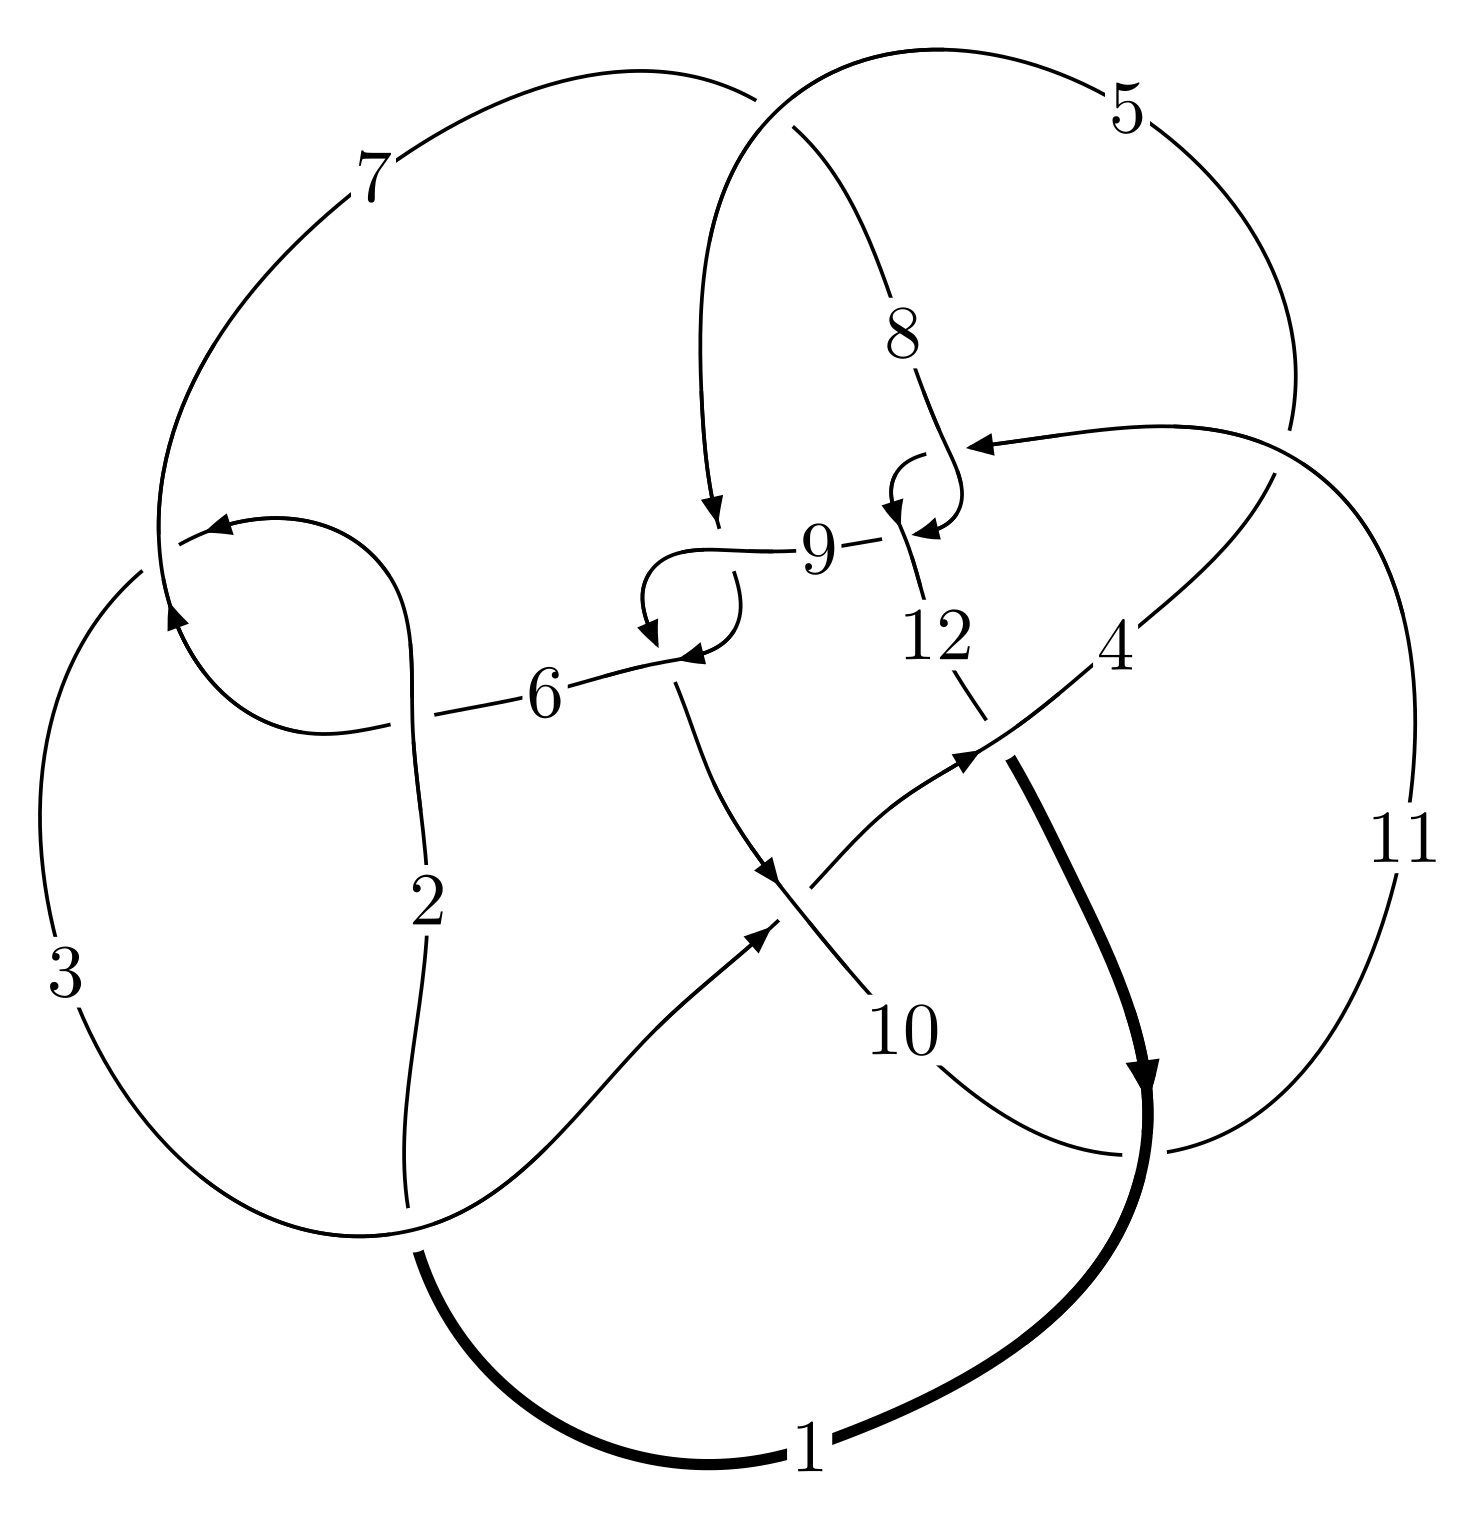
\includegraphics[width=112pt]{../../../GIT/diagram.site/Diagrams/png/1446_12a_0645.png}\\
\ \ \ A knot diagram\footnotemark}&
\allowdisplaybreaks
\textbf{Linearized knot diagam} \\
\cline{2-2}
 &
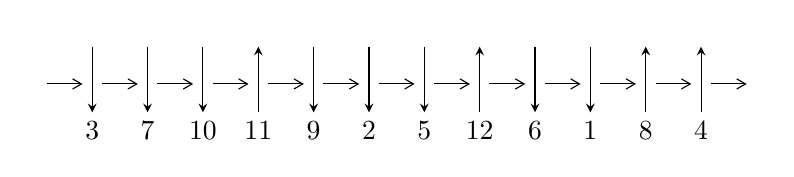
\begin{tikzpicture}[x=20pt, y=17pt]
	% nodes
	\node (C0) at (0, 0) {};
	\node (C1) at (1, 0) {};
	\node (C1U) at (1, +1) {};
	\node (C1D) at (1, -1) {3};

	\node (C2) at (2, 0) {};
	\node (C2U) at (2, +1) {};
	\node (C2D) at (2, -1) {7};

	\node (C3) at (3, 0) {};
	\node (C3U) at (3, +1) {};
	\node (C3D) at (3, -1) {10};

	\node (C4) at (4, 0) {};
	\node (C4U) at (4, +1) {};
	\node (C4D) at (4, -1) {11};

	\node (C5) at (5, 0) {};
	\node (C5U) at (5, +1) {};
	\node (C5D) at (5, -1) {9};

	\node (C6) at (6, 0) {};
	\node (C6U) at (6, +1) {};
	\node (C6D) at (6, -1) {2};

	\node (C7) at (7, 0) {};
	\node (C7U) at (7, +1) {};
	\node (C7D) at (7, -1) {5};

	\node (C8) at (8, 0) {};
	\node (C8U) at (8, +1) {};
	\node (C8D) at (8, -1) {12};

	\node (C9) at (9, 0) {};
	\node (C9U) at (9, +1) {};
	\node (C9D) at (9, -1) {6};

	\node (C10) at (10, 0) {};
	\node (C10U) at (10, +1) {};
	\node (C10D) at (10, -1) {1};

	\node (C11) at (11, 0) {};
	\node (C11U) at (11, +1) {};
	\node (C11D) at (11, -1) {8};

	\node (C12) at (12, 0) {};
	\node (C12U) at (12, +1) {};
	\node (C12D) at (12, -1) {4};
	\node (C13) at (13, 0) {};

	% arrows
	\draw[->,>={angle 60}]
	(C0) edge (C1) (C1) edge (C2) (C2) edge (C3) (C3) edge (C4) (C4) edge (C5) (C5) edge (C6) (C6) edge (C7) (C7) edge (C8) (C8) edge (C9) (C9) edge (C10) (C10) edge (C11) (C11) edge (C12) (C12) edge (C13) ;	\draw[->,>=stealth]
	(C1U) edge (C1D) (C2U) edge (C2D) (C3U) edge (C3D) (C4D) edge (C4U) (C5U) edge (C5D) (C6U) edge (C6D) (C7U) edge (C7D) (C8D) edge (C8U) (C9U) edge (C9D) (C10U) edge (C10D) (C11D) edge (C11U) (C12D) edge (C12U) ;
	\end{tikzpicture} \\
\hhline{~~} \\& 
\textbf{Solving Sequence} \\ \cline{2-2} 
 &
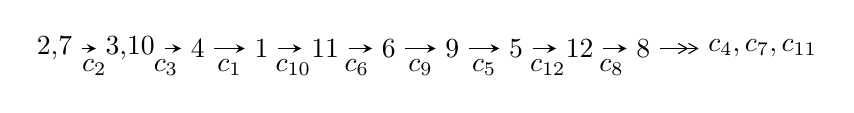
\begin{tikzpicture}[x=23pt, y=7pt]
	% node
	\node (A0) at (-1/8, 0) {2,7};
	\node (A1) at (17/16, 0) {3,10};
	\node (A2) at (17/8, 0) {4};
	\node (A3) at (25/8, 0) {1};
	\node (A4) at (33/8, 0) {11};
	\node (A5) at (41/8, 0) {6};
	\node (A6) at (49/8, 0) {9};
	\node (A7) at (57/8, 0) {5};
	\node (A8) at (65/8, 0) {12};
	\node (A9) at (73/8, 0) {8};
	\node (C1) at (1/2, -1) {$c_{2}$};
	\node (C2) at (13/8, -1) {$c_{3}$};
	\node (C3) at (21/8, -1) {$c_{1}$};
	\node (C4) at (29/8, -1) {$c_{10}$};
	\node (C5) at (37/8, -1) {$c_{6}$};
	\node (C6) at (45/8, -1) {$c_{9}$};
	\node (C7) at (53/8, -1) {$c_{5}$};
	\node (C8) at (61/8, -1) {$c_{12}$};
	\node (C9) at (69/8, -1) {$c_{8}$};
	\node (A10) at (11, 0) {$c_{4},c_{7},c_{11}$};

	% edge
	\draw[->,>=stealth]	
	(A0) edge (A1) (A1) edge (A2) (A2) edge (A3) (A3) edge (A4) (A4) edge (A5) (A5) edge (A6) (A6) edge (A7) (A7) edge (A8) (A8) edge (A9) ;
	\draw[->>,>={angle 60}]	
	(A9) edge (A10);
\end{tikzpicture} \\ 

\end{tabular} \\

\footnotetext{
The image of knot diagram is generated by the software ``\textbf{Draw programme}" developed by Andrew Bartholomew(\url{http://www.layer8.co.uk/maths/draw/index.htm\#Running-draw}), where we modified some parts for our purpose(\url{https://github.com/CATsTAILs/LinksPainter}).
}\phantom \\ \newline 
\centering \textbf{Ideals for irreducible components\footnotemark of $X_{\text{par}}$} 
 
\begin{align*}
I^u_{1}&=\langle 
-2.97362\times10^{478} u^{159}+7.20508\times10^{478} u^{158}+\cdots+4.01845\times10^{476} b-1.56559\times10^{480},\\
\phantom{I^u_{1}}&\phantom{= \langle  }-3.29775\times10^{480} u^{159}+6.08538\times10^{480} u^{158}+\cdots+7.75561\times10^{478} a-2.13475\times10^{482},\\
\phantom{I^u_{1}}&\phantom{= \langle  }3 u^{160}- u^{159}+\cdots+331 u+193\rangle \\
I^u_{2}&=\langle 
212681736 u^{30}-995826957 u^{29}+\cdots+135981283 b+1205561889,\\
\phantom{I^u_{2}}&\phantom{= \langle  }4200084636 u^{30}-2960109407 u^{29}+\cdots+135981283 a+2781584870,\;3 u^{31}-4 u^{30}+\cdots+6 u-1\rangle \\
\\
\end{align*}
\raggedright * 2 irreducible components of $\dim_{\mathbb{C}}=0$, with total 191 representations.\\
\footnotetext{All coefficients of polynomials are rational numbers. But the coefficients are sometimes approximated in decimal forms when there is not enough margin.}
\newpage
\renewcommand{\arraystretch}{1}
\centering \section*{I. $I^u_{1}= \langle -2.97\times10^{478} u^{159}+7.21\times10^{478} u^{158}+\cdots+4.02\times10^{476} b-1.57\times10^{480},\;-3.30\times10^{480} u^{159}+6.09\times10^{480} u^{158}+\cdots+7.76\times10^{478} a-2.13\times10^{482},\;3 u^{160}- u^{159}+\cdots+331 u+193 \rangle$}
\flushleft \textbf{(i) Arc colorings}\\
\begin{tabular}{m{7pt} m{180pt} m{7pt} m{180pt} }
\flushright $a_{2}=$&$\begin{pmatrix}1\\0\end{pmatrix}$ \\
\flushright $a_{7}=$&$\begin{pmatrix}0\\u\end{pmatrix}$ \\
\flushright $a_{3}=$&$\begin{pmatrix}1\\u^2\end{pmatrix}$ \\
\flushright $a_{10}=$&$\begin{pmatrix}42.5208 u^{159}-78.4642 u^{158}+\cdots+3808.29 u+2752.52\\73.9991 u^{159}-179.300 u^{158}+\cdots+8415.82 u+3896.00\end{pmatrix}$ \\
\flushright $a_{4}=$&$\begin{pmatrix}94.2155 u^{159}-135.360 u^{158}+\cdots+3663.40 u+3322.32\\74.6958 u^{159}-139.263 u^{158}+\cdots+2966.73 u+1181.62\end{pmatrix}$ \\
\flushright $a_{1}=$&$\begin{pmatrix}- u^2+1\\- u^4\end{pmatrix}$ \\
\flushright $a_{11}=$&$\begin{pmatrix}99.5335 u^{159}-156.029 u^{158}+\cdots+9476.32 u+7456.67\\140.093 u^{159}-275.547 u^{158}+\cdots+14805.5 u+8626.39\end{pmatrix}$ \\
\flushright $a_{6}=$&$\begin{pmatrix}u\\u\end{pmatrix}$ \\
\flushright $a_{9}=$&$\begin{pmatrix}123.309 u^{159}-190.843 u^{158}+\cdots+11751.0 u+8564.58\\154.787 u^{159}-291.679 u^{158}+\cdots+16358.6 u+9708.06\end{pmatrix}$ \\
\flushright $a_{5}=$&$\begin{pmatrix}53.1586 u^{159}-67.3439 u^{158}+\cdots+2128.47 u+2393.64\\43.2850 u^{159}-61.1105 u^{158}+\cdots+1169.30 u+903.031\end{pmatrix}$ \\
\flushright $a_{12}=$&$\begin{pmatrix}-149.073 u^{159}+163.399 u^{158}+\cdots-8258.49 u-11218.9\\-250.944 u^{159}+314.969 u^{158}+\cdots-13101.3 u-14923.1\end{pmatrix}$ \\
\flushright $a_{8}=$&$\begin{pmatrix}160.802 u^{159}-177.065 u^{158}+\cdots+9052.96 u+11563.7\\257.386 u^{159}-322.104 u^{158}+\cdots+13806.7 u+15180.7\end{pmatrix}$\\&\end{tabular}
\flushleft \textbf{(ii) Obstruction class $= -1$}\\~\\
\flushleft \textbf{(iii) Cusp Shapes $= -69.5462 u^{159}+85.0726 u^{158}+\cdots-2339.28 u-2896.34$}\\~\\
\newpage\renewcommand{\arraystretch}{1}
\flushleft \textbf{(iv) u-Polynomials at the component}\newline \\
\begin{tabular}{m{50pt}|m{274pt}}
Crossings & \hspace{64pt}u-Polynomials at each crossing \\
\hline $$\begin{aligned}c_{1}\end{aligned}$$&$\begin{aligned}
&9(9 u^{160}+625 u^{159}+\cdots+662313 u+37249)
\end{aligned}$\\
\hline $$\begin{aligned}c_{2},c_{6}\end{aligned}$$&$\begin{aligned}
&3(3 u^{160}+u^{159}+\cdots-331 u+193)
\end{aligned}$\\
\hline $$\begin{aligned}c_{3}\end{aligned}$$&$\begin{aligned}
&u^{160}+2 u^{159}+\cdots+138410 u+38043
\end{aligned}$\\
\hline $$\begin{aligned}c_{4}\end{aligned}$$&$\begin{aligned}
&u^{160}-3 u^{159}+\cdots+8419865 u-580297
\end{aligned}$\\
\hline $$\begin{aligned}c_{5},c_{9}\end{aligned}$$&$\begin{aligned}
&u^{160}-4 u^{159}+\cdots+5365970 u+823609
\end{aligned}$\\
\hline $$\begin{aligned}c_{7}\end{aligned}$$&$\begin{aligned}
&u^{160}-10 u^{159}+\cdots-10677820 u+828069
\end{aligned}$\\
\hline $$\begin{aligned}c_{8},c_{11}\end{aligned}$$&$\begin{aligned}
&3(3 u^{160}+7 u^{159}+\cdots+27391 u+4289)
\end{aligned}$\\
\hline $$\begin{aligned}c_{10}\end{aligned}$$&$\begin{aligned}
&u^{160}-6 u^{159}+\cdots-13655574 u+592191
\end{aligned}$\\
\hline $$\begin{aligned}c_{12}\end{aligned}$$&$\begin{aligned}
&9(9 u^{160}+139 u^{159}+\cdots+7244 u+959)
\end{aligned}$\\
\hline
\end{tabular}\\~\\
\newpage\renewcommand{\arraystretch}{1}
\flushleft \textbf{(v) Riley Polynomials at the component}\newline \\
\begin{tabular}{m{50pt}|m{274pt}}
Crossings & \hspace{64pt}Riley Polynomials at each crossing \\
\hline $$\begin{aligned}c_{1}\end{aligned}$$&$\begin{aligned}
&81(81 y^{160}+2819 y^{159}+\cdots+7.77369\times10^{11} y+1.38749\times10^{9})
\end{aligned}$\\
\hline $$\begin{aligned}c_{2},c_{6}\end{aligned}$$&$\begin{aligned}
&9(9 y^{160}-625 y^{159}+\cdots-662313 y+37249)
\end{aligned}$\\
\hline $$\begin{aligned}c_{3}\end{aligned}$$&$\begin{aligned}
&y^{160}-10 y^{159}+\cdots+181994273540 y+1447269849
\end{aligned}$\\
\hline $$\begin{aligned}c_{4}\end{aligned}$$&$\begin{aligned}
&y^{160}-7 y^{159}+\cdots-29142125376523 y+336744608209
\end{aligned}$\\
\hline $$\begin{aligned}c_{5},c_{9}\end{aligned}$$&$\begin{aligned}
&y^{160}-76 y^{159}+\cdots-6823756896730 y+678331784881
\end{aligned}$\\
\hline $$\begin{aligned}c_{7}\end{aligned}$$&$\begin{aligned}
&y^{160}+22 y^{159}+\cdots+33389274231554 y+685698268761
\end{aligned}$\\
\hline $$\begin{aligned}c_{8},c_{11}\end{aligned}$$&$\begin{aligned}
&9(9 y^{160}-787 y^{159}+\cdots-5.87148\times10^{8} y+1.83955\times10^{7})
\end{aligned}$\\
\hline $$\begin{aligned}c_{10}\end{aligned}$$&$\begin{aligned}
&y^{160}+6 y^{159}+\cdots+12702120885144 y+350690180481
\end{aligned}$\\
\hline $$\begin{aligned}c_{12}\end{aligned}$$&$\begin{aligned}
&81(81 y^{160}-583 y^{159}+\cdots-1.15876\times10^{7} y+919681)
\end{aligned}$\\
\hline
\end{tabular}\\~\\
\newpage\flushleft \textbf{(vi) Complex Volumes and Cusp Shapes}
$$\begin{array}{c|c|c}  
\text{Solutions to }I^u_{1}& \I (\text{vol} + \sqrt{-1}CS) & \text{Cusp shape}\\
 \hline 
\begin{aligned}
u &= -0.858523 + 0.512712 I \\
a &= \phantom{-}1.50494 + 4.91958 I \\
b &= \phantom{-}5.05179 + 1.41604 I\end{aligned}
 & -0.20205 + 2.08088 I & \phantom{-0.000000 } 0 \\ \hline\begin{aligned}
u &= -0.858523 - 0.512712 I \\
a &= \phantom{-}1.50494 - 4.91958 I \\
b &= \phantom{-}5.05179 - 1.41604 I\end{aligned}
 & -0.20205 - 2.08088 I & \phantom{-0.000000 } 0 \\ \hline\begin{aligned}
u &= -0.399566 + 0.920691 I \\
a &= -0.653839 - 0.918014 I \\
b &= -0.927677 + 0.110718 I\end{aligned}
 & \phantom{-}5.92805 - 3.86382 I & \phantom{-0.000000 } 0 \\ \hline\begin{aligned}
u &= -0.399566 - 0.920691 I \\
a &= -0.653839 + 0.918014 I \\
b &= -0.927677 - 0.110718 I\end{aligned}
 & \phantom{-}5.92805 + 3.86382 I & \phantom{-0.000000 } 0 \\ \hline\begin{aligned}
u &= -0.890101 + 0.442528 I \\
a &= \phantom{-}0.766212 + 0.910700 I \\
b &= -0.494498 + 0.090076 I\end{aligned}
 & -3.91659 + 3.92649 I & \phantom{-0.000000 } 0 \\ \hline\begin{aligned}
u &= -0.890101 - 0.442528 I \\
a &= \phantom{-}0.766212 - 0.910700 I \\
b &= -0.494498 - 0.090076 I\end{aligned}
 & -3.91659 - 3.92649 I & \phantom{-0.000000 } 0 \\ \hline\begin{aligned}
u &= \phantom{-}0.345258 + 0.919207 I \\
a &= \phantom{-}0.514884 - 1.212210 I \\
b &= \phantom{-}0.559264 + 0.062755 I\end{aligned}
 & \phantom{-}4.64153 + 5.08652 I & \phantom{-0.000000 } 0 \\ \hline\begin{aligned}
u &= \phantom{-}0.345258 - 0.919207 I \\
a &= \phantom{-}0.514884 + 1.212210 I \\
b &= \phantom{-}0.559264 - 0.062755 I\end{aligned}
 & \phantom{-}4.64153 - 5.08652 I & \phantom{-0.000000 } 0 \\ \hline\begin{aligned}
u &= -0.876818 + 0.441280 I \\
a &= \phantom{-}0.037704 - 0.249262 I \\
b &= \phantom{-}1.44747 + 0.47428 I\end{aligned}
 & -3.87061 - 0.30555 I & \phantom{-0.000000 } 0 \\ \hline\begin{aligned}
u &= -0.876818 - 0.441280 I \\
a &= \phantom{-}0.037704 + 0.249262 I \\
b &= \phantom{-}1.44747 - 0.47428 I\end{aligned}
 & -3.87061 + 0.30555 I & \phantom{-0.000000 } 0\\
 \hline 
 \end{array}$$\newpage$$\begin{array}{c|c|c}  
\text{Solutions to }I^u_{1}& \I (\text{vol} + \sqrt{-1}CS) & \text{Cusp shape}\\
 \hline 
\begin{aligned}
u &= \phantom{-}0.598820 + 0.765579 I \\
a &= -0.582350 + 1.040930 I \\
b &= -1.66724 + 0.31489 I\end{aligned}
 & \phantom{-}6.42128 + 7.98934 I & \phantom{-0.000000 } 0 \\ \hline\begin{aligned}
u &= \phantom{-}0.598820 - 0.765579 I \\
a &= -0.582350 - 1.040930 I \\
b &= -1.66724 - 0.31489 I\end{aligned}
 & \phantom{-}6.42128 - 7.98934 I & \phantom{-0.000000 } 0 \\ \hline\begin{aligned}
u &= \phantom{-}0.875198 + 0.546004 I \\
a &= \phantom{-}2.33898 + 1.12309 I \\
b &= \phantom{-}0.05287 + 2.88551 I\end{aligned}
 & -0.08564 - 1.61768 I & \phantom{-0.000000 } 0 \\ \hline\begin{aligned}
u &= \phantom{-}0.875198 - 0.546004 I \\
a &= \phantom{-}2.33898 - 1.12309 I \\
b &= \phantom{-}0.05287 - 2.88551 I\end{aligned}
 & -0.08564 + 1.61768 I & \phantom{-0.000000 } 0 \\ \hline\begin{aligned}
u &= \phantom{-}0.599472 + 0.755917 I \\
a &= \phantom{-}0.536468 - 0.671135 I \\
b &= \phantom{-}1.379940 - 0.295092 I\end{aligned}
 & \phantom{-}2.52740 + 3.16960 I & \phantom{-0.000000 } 0 \\ \hline\begin{aligned}
u &= \phantom{-}0.599472 - 0.755917 I \\
a &= \phantom{-}0.536468 + 0.671135 I \\
b &= \phantom{-}1.379940 + 0.295092 I\end{aligned}
 & \phantom{-}2.52740 - 3.16960 I & \phantom{-0.000000 } 0 \\ \hline\begin{aligned}
u &= -0.875532 + 0.402402 I \\
a &= -1.32734 - 1.50867 I \\
b &= -2.14051 - 2.03517 I\end{aligned}
 & \phantom{-}1.20283 - 5.35350 I & \phantom{-0.000000 } 0 \\ \hline\begin{aligned}
u &= -0.875532 - 0.402402 I \\
a &= -1.32734 + 1.50867 I \\
b &= -2.14051 + 2.03517 I\end{aligned}
 & \phantom{-}1.20283 + 5.35350 I & \phantom{-0.000000 } 0 \\ \hline\begin{aligned}
u &= \phantom{-}0.520979 + 0.809128 I \\
a &= -1.44567 + 0.74943 I \\
b &= -1.051720 - 0.592214 I\end{aligned}
 & -2.00969 + 2.22775 I & \phantom{-0.000000 } 0 \\ \hline\begin{aligned}
u &= \phantom{-}0.520979 - 0.809128 I \\
a &= -1.44567 - 0.74943 I \\
b &= -1.051720 + 0.592214 I\end{aligned}
 & -2.00969 - 2.22775 I & \phantom{-0.000000 } 0\\
 \hline 
 \end{array}$$\newpage$$\begin{array}{c|c|c}  
\text{Solutions to }I^u_{1}& \I (\text{vol} + \sqrt{-1}CS) & \text{Cusp shape}\\
 \hline 
\begin{aligned}
u &= \phantom{-}0.964376 + 0.391414 I \\
a &= \phantom{-}0.210562 - 1.129790 I \\
b &= \phantom{-}0.517869 - 0.633031 I\end{aligned}
 & -2.32367 - 1.28895 I & \phantom{-0.000000 } 0 \\ \hline\begin{aligned}
u &= \phantom{-}0.964376 - 0.391414 I \\
a &= \phantom{-}0.210562 + 1.129790 I \\
b &= \phantom{-}0.517869 + 0.633031 I\end{aligned}
 & -2.32367 + 1.28895 I & \phantom{-0.000000 } 0 \\ \hline\begin{aligned}
u &= \phantom{-}0.598126 + 0.749447 I \\
a &= -0.018088 + 0.669995 I \\
b &= -1.243940 + 0.671685 I\end{aligned}
 & \phantom{-}6.43884 - 1.85606 I & \phantom{-0.000000 } 0 \\ \hline\begin{aligned}
u &= \phantom{-}0.598126 - 0.749447 I \\
a &= -0.018088 - 0.669995 I \\
b &= -1.243940 - 0.671685 I\end{aligned}
 & \phantom{-}6.43884 + 1.85606 I & \phantom{-0.000000 } 0 \\ \hline\begin{aligned}
u &= -0.856928 + 0.415771 I \\
a &= \phantom{-}0.88931 + 1.26976 I \\
b &= \phantom{-}1.93123 + 1.58580 I\end{aligned}
 & -1.65691 - 0.86452 I & \phantom{-0.000000 } 0 \\ \hline\begin{aligned}
u &= -0.856928 - 0.415771 I \\
a &= \phantom{-}0.88931 - 1.26976 I \\
b &= \phantom{-}1.93123 - 1.58580 I\end{aligned}
 & -1.65691 + 0.86452 I & \phantom{-0.000000 } 0 \\ \hline\begin{aligned}
u &= -0.806252 + 0.506145 I \\
a &= -0.87444 - 1.57282 I \\
b &= -1.56031 - 0.99865 I\end{aligned}
 & \phantom{-}1.74273 + 2.08497 I & \phantom{-0.000000 } 0 \\ \hline\begin{aligned}
u &= -0.806252 - 0.506145 I \\
a &= -0.87444 + 1.57282 I \\
b &= -1.56031 + 0.99865 I\end{aligned}
 & \phantom{-}1.74273 - 2.08497 I & \phantom{-0.000000 } 0 \\ \hline\begin{aligned}
u &= \phantom{-}0.535100 + 0.785517 I \\
a &= \phantom{-}1.47924 - 0.88491 I \\
b &= \phantom{-}1.36629 + 0.50675 I\end{aligned}
 & -1.01099 + 5.78248 I & \phantom{-0.000000 } 0 \\ \hline\begin{aligned}
u &= \phantom{-}0.535100 - 0.785517 I \\
a &= \phantom{-}1.47924 + 0.88491 I \\
b &= \phantom{-}1.36629 - 0.50675 I\end{aligned}
 & -1.01099 - 5.78248 I & \phantom{-0.000000 } 0\\
 \hline 
 \end{array}$$\newpage$$\begin{array}{c|c|c}  
\text{Solutions to }I^u_{1}& \I (\text{vol} + \sqrt{-1}CS) & \text{Cusp shape}\\
 \hline 
\begin{aligned}
u &= -0.626179 + 0.843667 I \\
a &= \phantom{-}0.169285 + 0.779136 I \\
b &= \phantom{-}0.946759 + 0.496073 I\end{aligned}
 & \phantom{-}7.45083 - 0.28837 I & \phantom{-0.000000 } 0 \\ \hline\begin{aligned}
u &= -0.626179 - 0.843667 I \\
a &= \phantom{-}0.169285 - 0.779136 I \\
b &= \phantom{-}0.946759 - 0.496073 I\end{aligned}
 & \phantom{-}7.45083 + 0.28837 I & \phantom{-0.000000 } 0 \\ \hline\begin{aligned}
u &= -0.948712 + 0.454402 I \\
a &= \phantom{-}1.40790 + 1.16283 I \\
b &= \phantom{-}1.021270 + 0.497104 I\end{aligned}
 & -2.04324 + 4.34407 I & \phantom{-0.000000 } 0 \\ \hline\begin{aligned}
u &= -0.948712 - 0.454402 I \\
a &= \phantom{-}1.40790 - 1.16283 I \\
b &= \phantom{-}1.021270 - 0.497104 I\end{aligned}
 & -2.04324 - 4.34407 I & \phantom{-0.000000 } 0 \\ \hline\begin{aligned}
u &= -0.931616 + 0.500567 I \\
a &= -1.22621 - 1.87235 I \\
b &= -2.01752 - 0.73224 I\end{aligned}
 & \phantom{-}1.46381 + 1.84510 I & \phantom{-0.000000 } 0 \\ \hline\begin{aligned}
u &= -0.931616 - 0.500567 I \\
a &= -1.22621 + 1.87235 I \\
b &= -2.01752 + 0.73224 I\end{aligned}
 & \phantom{-}1.46381 - 1.84510 I & \phantom{-0.000000 } 0 \\ \hline\begin{aligned}
u &= -0.776028 + 0.723624 I \\
a &= -0.916415 - 0.514421 I \\
b &= -1.273670 - 0.057649 I\end{aligned}
 & \phantom{-}2.88771 + 1.95925 I & \phantom{-0.000000 } 0 \\ \hline\begin{aligned}
u &= -0.776028 - 0.723624 I \\
a &= -0.916415 + 0.514421 I \\
b &= -1.273670 + 0.057649 I\end{aligned}
 & \phantom{-}2.88771 - 1.95925 I & \phantom{-0.000000 } 0 \\ \hline\begin{aligned}
u &= \phantom{-}0.755572 + 0.545167 I \\
a &= \phantom{-}1.68045 - 2.03588 I \\
b &= \phantom{-}1.061500 - 0.844023 I\end{aligned}
 & \phantom{-}2.75731 + 5.54693 I & \phantom{-0.000000 } 0 \\ \hline\begin{aligned}
u &= \phantom{-}0.755572 - 0.545167 I \\
a &= \phantom{-}1.68045 + 2.03588 I \\
b &= \phantom{-}1.061500 + 0.844023 I\end{aligned}
 & \phantom{-}2.75731 - 5.54693 I & \phantom{-0.000000 } 0\\
 \hline 
 \end{array}$$\newpage$$\begin{array}{c|c|c}  
\text{Solutions to }I^u_{1}& \I (\text{vol} + \sqrt{-1}CS) & \text{Cusp shape}\\
 \hline 
\begin{aligned}
u &= \phantom{-}0.759372 + 0.531679 I \\
a &= \phantom{-}0.43982 - 1.78428 I \\
b &= \phantom{-}0.003159 - 0.785364 I\end{aligned}
 & \phantom{-}3.59006 - 2.57418 I & \phantom{-0.000000 } 0 \\ \hline\begin{aligned}
u &= \phantom{-}0.759372 - 0.531679 I \\
a &= \phantom{-}0.43982 + 1.78428 I \\
b &= \phantom{-}0.003159 + 0.785364 I\end{aligned}
 & \phantom{-}3.59006 + 2.57418 I & \phantom{-0.000000 } 0 \\ \hline\begin{aligned}
u &= \phantom{-}0.921773 + 0.554518 I \\
a &= \phantom{-}0.847379 + 0.063602 I \\
b &= \phantom{-}1.72736 - 0.21624 I\end{aligned}
 & \phantom{-}3.05691 - 1.82766 I & \phantom{-0.000000 } 0 \\ \hline\begin{aligned}
u &= \phantom{-}0.921773 - 0.554518 I \\
a &= \phantom{-}0.847379 - 0.063602 I \\
b &= \phantom{-}1.72736 + 0.21624 I\end{aligned}
 & \phantom{-}3.05691 + 1.82766 I & \phantom{-0.000000 } 0 \\ \hline\begin{aligned}
u &= -0.482878 + 0.961506 I \\
a &= -1.143840 - 0.828686 I \\
b &= -1.083810 + 0.554385 I\end{aligned}
 & \phantom{-}2.4349 - 14.4432 I & \phantom{-0.000000 } 0 \\ \hline\begin{aligned}
u &= -0.482878 - 0.961506 I \\
a &= -1.143840 + 0.828686 I \\
b &= -1.083810 - 0.554385 I\end{aligned}
 & \phantom{-}2.4349 + 14.4432 I & \phantom{-0.000000 } 0 \\ \hline\begin{aligned}
u &= \phantom{-}0.929044 + 0.546307 I \\
a &= -0.889605 + 0.899784 I \\
b &= -2.00277 + 1.23026 I\end{aligned}
 & -0.67270 - 5.34745 I & \phantom{-0.000000 } 0 \\ \hline\begin{aligned}
u &= \phantom{-}0.929044 - 0.546307 I \\
a &= -0.889605 - 0.899784 I \\
b &= -2.00277 - 1.23026 I\end{aligned}
 & -0.67270 + 5.34745 I & \phantom{-0.000000 } 0 \\ \hline\begin{aligned}
u &= \phantom{-}0.929136 + 0.547891 I \\
a &= \phantom{-}1.52833 - 0.96048 I \\
b &= \phantom{-}2.69093 - 1.18841 I\end{aligned}
 & \phantom{-}2.19729 - 9.95091 I & \phantom{-0.000000 } 0 \\ \hline\begin{aligned}
u &= \phantom{-}0.929136 - 0.547891 I \\
a &= \phantom{-}1.52833 + 0.96048 I \\
b &= \phantom{-}2.69093 + 1.18841 I\end{aligned}
 & \phantom{-}2.19729 + 9.95091 I & \phantom{-0.000000 } 0\\
 \hline 
 \end{array}$$\newpage$$\begin{array}{c|c|c}  
\text{Solutions to }I^u_{1}& \I (\text{vol} + \sqrt{-1}CS) & \text{Cusp shape}\\
 \hline 
\begin{aligned}
u &= -1.004960 + 0.399803 I \\
a &= -1.40868 - 0.88746 I \\
b &= -1.099750 - 0.855542 I\end{aligned}
 & \phantom{-}0.88846 + 8.43462 I & \phantom{-0.000000 } 0 \\ \hline\begin{aligned}
u &= -1.004960 - 0.399803 I \\
a &= -1.40868 + 0.88746 I \\
b &= -1.099750 + 0.855542 I\end{aligned}
 & \phantom{-}0.88846 - 8.43462 I & \phantom{-0.000000 } 0 \\ \hline\begin{aligned}
u &= \phantom{-}0.738735 + 0.536581 I \\
a &= -1.33873 + 1.44316 I \\
b &= -0.690771 + 0.374518 I\end{aligned}
 & -0.072951 + 0.961480 I & \phantom{-0.000000 } 0 \\ \hline\begin{aligned}
u &= \phantom{-}0.738735 - 0.536581 I \\
a &= -1.33873 - 1.44316 I \\
b &= -0.690771 - 0.374518 I\end{aligned}
 & -0.072951 - 0.961480 I & \phantom{-0.000000 } 0 \\ \hline\begin{aligned}
u &= -0.854118 + 0.679305 I \\
a &= -0.15786 + 1.91806 I \\
b &= \phantom{-}0.62577 + 1.61923 I\end{aligned}
 & \phantom{-}4.81237 - 0.44211 I & \phantom{-0.000000 } 0 \\ \hline\begin{aligned}
u &= -0.854118 - 0.679305 I \\
a &= -0.15786 - 1.91806 I \\
b &= \phantom{-}0.62577 - 1.61923 I\end{aligned}
 & \phantom{-}4.81237 + 0.44211 I & \phantom{-0.000000 } 0 \\ \hline\begin{aligned}
u &= -0.466443 + 0.987944 I \\
a &= \phantom{-}0.991951 + 0.705897 I \\
b &= \phantom{-}0.932721 - 0.503111 I\end{aligned}
 & -0.60239 - 8.18752 I & \phantom{-0.000000 } 0 \\ \hline\begin{aligned}
u &= -0.466443 - 0.987944 I \\
a &= \phantom{-}0.991951 - 0.705897 I \\
b &= \phantom{-}0.932721 + 0.503111 I\end{aligned}
 & -0.60239 + 8.18752 I & \phantom{-0.000000 } 0 \\ \hline\begin{aligned}
u &= \phantom{-}0.957099 + 0.540908 I \\
a &= \phantom{-}0.14141 + 1.66823 I \\
b &= -0.99477 + 2.04946 I\end{aligned}
 & -3.01144 - 4.92489 I & \phantom{-0.000000 } 0 \\ \hline\begin{aligned}
u &= \phantom{-}0.957099 - 0.540908 I \\
a &= \phantom{-}0.14141 - 1.66823 I \\
b &= -0.99477 - 2.04946 I\end{aligned}
 & -3.01144 + 4.92489 I & \phantom{-0.000000 } 0\\
 \hline 
 \end{array}$$\newpage$$\begin{array}{c|c|c}  
\text{Solutions to }I^u_{1}& \I (\text{vol} + \sqrt{-1}CS) & \text{Cusp shape}\\
 \hline 
\begin{aligned}
u &= -1.108390 + 0.036148 I \\
a &= \phantom{-}0.412788 + 0.414387 I \\
b &= -0.813571 + 0.037760 I\end{aligned}
 & -6.57571 - 4.32904 I & \phantom{-0.000000 } 0 \\ \hline\begin{aligned}
u &= -1.108390 - 0.036148 I \\
a &= \phantom{-}0.412788 - 0.414387 I \\
b &= -0.813571 - 0.037760 I\end{aligned}
 & -6.57571 + 4.32904 I & \phantom{-0.000000 } 0 \\ \hline\begin{aligned}
u &= \phantom{-}0.721883 + 0.511371 I \\
a &= -1.76456 + 0.10147 I \\
b &= -0.49151 - 1.64811 I\end{aligned}
 & \phantom{-}0.30418 - 2.77851 I & \phantom{-0.000000 } 0 \\ \hline\begin{aligned}
u &= \phantom{-}0.721883 - 0.511371 I \\
a &= -1.76456 - 0.10147 I \\
b &= -0.49151 + 1.64811 I\end{aligned}
 & \phantom{-}0.30418 + 2.77851 I & \phantom{-0.000000 } 0 \\ \hline\begin{aligned}
u &= \phantom{-}0.995347 + 0.504511 I \\
a &= -0.32124 - 1.51056 I \\
b &= \phantom{-}0.50761 - 1.70473 I\end{aligned}
 & -3.11466 - 1.07906 I & \phantom{-0.000000 } 0 \\ \hline\begin{aligned}
u &= \phantom{-}0.995347 - 0.504511 I \\
a &= -0.32124 + 1.51056 I \\
b &= \phantom{-}0.50761 + 1.70473 I\end{aligned}
 & -3.11466 + 1.07906 I & \phantom{-0.000000 } 0 \\ \hline\begin{aligned}
u &= -0.868062 + 0.709058 I \\
a &= \phantom{-}1.57283 - 0.12343 I \\
b &= \phantom{-}1.63720 - 0.80832 I\end{aligned}
 & \phantom{-}4.78608 + 5.78377 I & \phantom{-0.000000 } 0 \\ \hline\begin{aligned}
u &= -0.868062 - 0.709058 I \\
a &= \phantom{-}1.57283 + 0.12343 I \\
b &= \phantom{-}1.63720 + 0.80832 I\end{aligned}
 & \phantom{-}4.78608 - 5.78377 I & \phantom{-0.000000 } 0 \\ \hline\begin{aligned}
u &= -0.870669 + 0.080722 I \\
a &= \phantom{-}1.24479 + 1.41373 I \\
b &= \phantom{-}0.680066 + 0.603111 I\end{aligned}
 & -2.39934 - 2.95807 I & \phantom{-0.000000 } 0 \\ \hline\begin{aligned}
u &= -0.870669 - 0.080722 I \\
a &= \phantom{-}1.24479 - 1.41373 I \\
b &= \phantom{-}0.680066 - 0.603111 I\end{aligned}
 & -2.39934 + 2.95807 I & \phantom{-0.000000 } 0\\
 \hline 
 \end{array}$$\newpage$$\begin{array}{c|c|c}  
\text{Solutions to }I^u_{1}& \I (\text{vol} + \sqrt{-1}CS) & \text{Cusp shape}\\
 \hline 
\begin{aligned}
u &= -1.115030 + 0.177294 I \\
a &= -0.216775 + 0.957878 I \\
b &= -1.30923 + 0.81369 I\end{aligned}
 & -5.24468 + 0.22869 I & \phantom{-0.000000 } 0 \\ \hline\begin{aligned}
u &= -1.115030 - 0.177294 I \\
a &= -0.216775 - 0.957878 I \\
b &= -1.30923 - 0.81369 I\end{aligned}
 & -5.24468 - 0.22869 I & \phantom{-0.000000 } 0 \\ \hline\begin{aligned}
u &= \phantom{-}0.420181 + 0.759965 I \\
a &= -1.63220 + 1.14348 I \\
b &= -1.003700 - 0.159361 I\end{aligned}
 & -0.65932 + 4.36442 I & \phantom{-0.000000 } 0 \\ \hline\begin{aligned}
u &= \phantom{-}0.420181 - 0.759965 I \\
a &= -1.63220 - 1.14348 I \\
b &= -1.003700 + 0.159361 I\end{aligned}
 & -0.65932 - 4.36442 I & \phantom{-0.000000 } 0 \\ \hline\begin{aligned}
u &= -0.816509 + 0.287001 I \\
a &= -1.18022 - 1.97542 I \\
b &= -1.58080 - 0.88820 I\end{aligned}
 & \phantom{-}2.11286 + 1.69342 I & \phantom{-0.000000 } 0 \\ \hline\begin{aligned}
u &= -0.816509 - 0.287001 I \\
a &= -1.18022 + 1.97542 I \\
b &= -1.58080 + 0.88820 I\end{aligned}
 & \phantom{-}2.11286 - 1.69342 I & \phantom{-0.000000 } 0 \\ \hline\begin{aligned}
u &= -0.819864 + 0.266572 I \\
a &= -0.62318 - 1.90819 I \\
b &= -0.80637 - 1.78729 I\end{aligned}
 & \phantom{-}1.51246 + 2.50065 I & \phantom{-0.000000 } 0 \\ \hline\begin{aligned}
u &= -0.819864 - 0.266572 I \\
a &= -0.62318 + 1.90819 I \\
b &= -0.80637 + 1.78729 I\end{aligned}
 & \phantom{-}1.51246 - 2.50065 I & \phantom{-0.000000 } 0 \\ \hline\begin{aligned}
u &= \phantom{-}0.180802 + 0.842553 I \\
a &= -0.366372 - 0.969411 I \\
b &= \phantom{-}0.082429 - 0.379043 I\end{aligned}
 & \phantom{-}4.48198 - 5.22354 I & \phantom{-0.000000 } 0 \\ \hline\begin{aligned}
u &= \phantom{-}0.180802 - 0.842553 I \\
a &= -0.366372 + 0.969411 I \\
b &= \phantom{-}0.082429 + 0.379043 I\end{aligned}
 & \phantom{-}4.48198 + 5.22354 I & \phantom{-0.000000 } 0\\
 \hline 
 \end{array}$$\newpage$$\begin{array}{c|c|c}  
\text{Solutions to }I^u_{1}& \I (\text{vol} + \sqrt{-1}CS) & \text{Cusp shape}\\
 \hline 
\begin{aligned}
u &= -0.929349 + 0.664804 I \\
a &= -0.41692 - 1.36478 I \\
b &= -0.946883 - 0.937696 I\end{aligned}
 & \phantom{-}2.39145 + 3.35955 I & \phantom{-0.000000 } 0 \\ \hline\begin{aligned}
u &= -0.929349 - 0.664804 I \\
a &= -0.41692 + 1.36478 I \\
b &= -0.946883 + 0.937696 I\end{aligned}
 & \phantom{-}2.39145 - 3.35955 I & \phantom{-0.000000 } 0 \\ \hline\begin{aligned}
u &= \phantom{-}0.480582 + 0.701769 I \\
a &= \phantom{-}1.74886 - 0.70670 I \\
b &= \phantom{-}1.164280 + 0.135179 I\end{aligned}
 & -0.60338 + 1.74935 I & \phantom{-0.000000 } 0 \\ \hline\begin{aligned}
u &= \phantom{-}0.480582 - 0.701769 I \\
a &= \phantom{-}1.74886 + 0.70670 I \\
b &= \phantom{-}1.164280 - 0.135179 I\end{aligned}
 & -0.60338 - 1.74935 I & \phantom{-0.000000 } 0 \\ \hline\begin{aligned}
u &= -1.164650 + 0.035527 I \\
a &= -0.160183 - 0.210952 I \\
b &= \phantom{-}1.083000 - 0.050934 I\end{aligned}
 & -7.78473 - 0.46269 I & \phantom{-0.000000 } 0 \\ \hline\begin{aligned}
u &= -1.164650 - 0.035527 I \\
a &= -0.160183 + 0.210952 I \\
b &= \phantom{-}1.083000 + 0.050934 I\end{aligned}
 & -7.78473 + 0.46269 I & \phantom{-0.000000 } 0 \\ \hline\begin{aligned}
u &= \phantom{-}0.565026 + 0.614392 I \\
a &= -1.41951 + 0.26683 I \\
b &= -0.541770 - 0.787177 I\end{aligned}
 & -1.95528 + 0.40890 I & \phantom{-0.000000 } 0 \\ \hline\begin{aligned}
u &= \phantom{-}0.565026 - 0.614392 I \\
a &= -1.41951 - 0.26683 I \\
b &= -0.541770 + 0.787177 I\end{aligned}
 & -1.95528 - 0.40890 I & \phantom{-0.000000 } 0 \\ \hline\begin{aligned}
u &= -0.839944 + 0.814312 I \\
a &= -1.04023 + 1.00033 I \\
b &= -0.35402 + 1.38938 I\end{aligned}
 & \phantom{-}3.86284 + 5.61334 I & \phantom{-0.000000 } 0 \\ \hline\begin{aligned}
u &= -0.839944 - 0.814312 I \\
a &= -1.04023 - 1.00033 I \\
b &= -0.35402 - 1.38938 I\end{aligned}
 & \phantom{-}3.86284 - 5.61334 I & \phantom{-0.000000 } 0\\
 \hline 
 \end{array}$$\newpage$$\begin{array}{c|c|c}  
\text{Solutions to }I^u_{1}& \I (\text{vol} + \sqrt{-1}CS) & \text{Cusp shape}\\
 \hline 
\begin{aligned}
u &= -0.827198 + 0.026035 I \\
a &= -1.73308 + 1.15402 I \\
b &= -0.880693 + 0.160135 I\end{aligned}
 & \phantom{-}1.05929 + 7.91977 I & \phantom{-0.000000 } 0 \\ \hline\begin{aligned}
u &= -0.827198 - 0.026035 I \\
a &= -1.73308 - 1.15402 I \\
b &= -0.880693 - 0.160135 I\end{aligned}
 & \phantom{-}1.05929 - 7.91977 I & \phantom{-0.000000 } 0 \\ \hline\begin{aligned}
u &= \phantom{-}1.147450 + 0.253250 I \\
a &= -0.613798 - 0.129454 I \\
b &= \phantom{-}0.468990 - 0.718982 I\end{aligned}
 & -3.98129 + 4.28687 I & \phantom{-0.000000 } 0 \\ \hline\begin{aligned}
u &= \phantom{-}1.147450 - 0.253250 I \\
a &= -0.613798 + 0.129454 I \\
b &= \phantom{-}0.468990 + 0.718982 I\end{aligned}
 & -3.98129 - 4.28687 I & \phantom{-0.000000 } 0 \\ \hline\begin{aligned}
u &= -1.177650 + 0.191619 I \\
a &= \phantom{-}0.510995 - 0.627460 I \\
b &= \phantom{-}1.66796 - 0.37807 I\end{aligned}
 & -5.59671 - 1.86006 I & \phantom{-0.000000 } 0 \\ \hline\begin{aligned}
u &= -1.177650 - 0.191619 I \\
a &= \phantom{-}0.510995 + 0.627460 I \\
b &= \phantom{-}1.66796 + 0.37807 I\end{aligned}
 & -5.59671 + 1.86006 I & \phantom{-0.000000 } 0 \\ \hline\begin{aligned}
u &= \phantom{-}0.764996 + 0.251400 I \\
a &= -1.38964 + 0.30977 I \\
b &= -0.432945 - 1.081040 I\end{aligned}
 & \phantom{-}0.32979 - 2.90045 I & \phantom{-0.000000 } 0 \\ \hline\begin{aligned}
u &= \phantom{-}0.764996 - 0.251400 I \\
a &= -1.38964 - 0.30977 I \\
b &= -0.432945 + 1.081040 I\end{aligned}
 & \phantom{-}0.32979 + 2.90045 I & \phantom{-0.000000 } 0 \\ \hline\begin{aligned}
u &= \phantom{-}1.024040 + 0.634235 I \\
a &= -0.959462 + 0.990982 I \\
b &= -1.003000 - 0.039725 I\end{aligned}
 & \phantom{-}5.14885 - 3.40949 I & \phantom{-0.000000 } 0 \\ \hline\begin{aligned}
u &= \phantom{-}1.024040 - 0.634235 I \\
a &= -0.959462 - 0.990982 I \\
b &= -1.003000 + 0.039725 I\end{aligned}
 & \phantom{-}5.14885 + 3.40949 I & \phantom{-0.000000 } 0\\
 \hline 
 \end{array}$$\newpage$$\begin{array}{c|c|c}  
\text{Solutions to }I^u_{1}& \I (\text{vol} + \sqrt{-1}CS) & \text{Cusp shape}\\
 \hline 
\begin{aligned}
u &= \phantom{-}1.029250 + 0.643230 I \\
a &= \phantom{-}0.80365 - 1.38739 I \\
b &= \phantom{-}1.218130 - 0.615126 I\end{aligned}
 & \phantom{-}1.22303 - 8.49093 I & \phantom{-0.000000 } 0 \\ \hline\begin{aligned}
u &= \phantom{-}1.029250 - 0.643230 I \\
a &= \phantom{-}0.80365 + 1.38739 I \\
b &= \phantom{-}1.218130 + 0.615126 I\end{aligned}
 & \phantom{-}1.22303 + 8.49093 I & \phantom{-0.000000 } 0 \\ \hline\begin{aligned}
u &= \phantom{-}1.028570 + 0.651156 I \\
a &= -1.02382 + 1.55998 I \\
b &= -1.70686 + 0.58162 I\end{aligned}
 & \phantom{-}5.1235 - 13.3621 I & \phantom{-0.000000 } 0 \\ \hline\begin{aligned}
u &= \phantom{-}1.028570 - 0.651156 I \\
a &= -1.02382 - 1.55998 I \\
b &= -1.70686 - 0.58162 I\end{aligned}
 & \phantom{-}5.1235 + 13.3621 I & \phantom{-0.000000 } 0 \\ \hline\begin{aligned}
u &= -1.091420 + 0.539497 I \\
a &= -0.28059 - 1.70796 I \\
b &= -1.63451 - 1.64993 I\end{aligned}
 & -2.11757 + 11.83540 I & \phantom{-0.000000 } 0 \\ \hline\begin{aligned}
u &= -1.091420 - 0.539497 I \\
a &= -0.28059 + 1.70796 I \\
b &= -1.63451 + 1.64993 I\end{aligned}
 & -2.11757 - 11.83540 I & \phantom{-0.000000 } 0 \\ \hline\begin{aligned}
u &= -0.917005 + 0.804673 I \\
a &= \phantom{-}1.010330 - 0.929796 I \\
b &= \phantom{-}0.51265 - 1.47019 I\end{aligned}
 & \phantom{-}3.63889 + 0.42575 I & \phantom{-0.000000 } 0 \\ \hline\begin{aligned}
u &= -0.917005 - 0.804673 I \\
a &= \phantom{-}1.010330 + 0.929796 I \\
b &= \phantom{-}0.51265 + 1.47019 I\end{aligned}
 & \phantom{-}3.63889 - 0.42575 I & \phantom{-0.000000 } 0 \\ \hline\begin{aligned}
u &= \phantom{-}1.218830 + 0.177949 I \\
a &= \phantom{-}0.067118 + 0.324108 I \\
b &= \phantom{-}0.385715 + 0.041239 I\end{aligned}
 & \phantom{-}0.226309 + 0.633517 I & \phantom{-0.000000 } 0 \\ \hline\begin{aligned}
u &= \phantom{-}1.218830 - 0.177949 I \\
a &= \phantom{-}0.067118 - 0.324108 I \\
b &= \phantom{-}0.385715 - 0.041239 I\end{aligned}
 & \phantom{-}0.226309 - 0.633517 I & \phantom{-0.000000 } 0\\
 \hline 
 \end{array}$$\newpage$$\begin{array}{c|c|c}  
\text{Solutions to }I^u_{1}& \I (\text{vol} + \sqrt{-1}CS) & \text{Cusp shape}\\
 \hline 
\begin{aligned}
u &= \phantom{-}1.070190 + 0.612135 I \\
a &= \phantom{-}0.49053 - 1.87768 I \\
b &= \phantom{-}1.23698 - 2.13388 I\end{aligned}
 & -2.32132 - 6.84418 I & \phantom{-0.000000 } 0 \\ \hline\begin{aligned}
u &= \phantom{-}1.070190 - 0.612135 I \\
a &= \phantom{-}0.49053 + 1.87768 I \\
b &= \phantom{-}1.23698 + 2.13388 I\end{aligned}
 & -2.32132 + 6.84418 I & \phantom{-0.000000 } 0 \\ \hline\begin{aligned}
u &= -1.132180 + 0.490877 I \\
a &= \phantom{-}0.47531 + 1.42514 I \\
b &= \phantom{-}1.52760 + 1.36159 I\end{aligned}
 & -5.42116 + 5.68279 I & \phantom{-0.000000 } 0 \\ \hline\begin{aligned}
u &= -1.132180 - 0.490877 I \\
a &= \phantom{-}0.47531 - 1.42514 I \\
b &= \phantom{-}1.52760 - 1.36159 I\end{aligned}
 & -5.42116 - 5.68279 I & \phantom{-0.000000 } 0 \\ \hline\begin{aligned}
u &= \phantom{-}0.424472 + 0.630167 I \\
a &= \phantom{-}1.264210 + 0.070425 I \\
b &= \phantom{-}0.367634 + 0.939807 I\end{aligned}
 & -1.49570 - 3.25862 I & \phantom{-0.000000 } 0 \\ \hline\begin{aligned}
u &= \phantom{-}0.424472 - 0.630167 I \\
a &= \phantom{-}1.264210 - 0.070425 I \\
b &= \phantom{-}0.367634 - 0.939807 I\end{aligned}
 & -1.49570 + 3.25862 I & \phantom{-0.000000 } 0 \\ \hline\begin{aligned}
u &= -1.025350 + 0.707689 I \\
a &= \phantom{-}0.677942 + 0.799775 I \\
b &= \phantom{-}1.048920 + 0.212449 I\end{aligned}
 & \phantom{-}6.24337 + 6.04898 I & \phantom{-0.000000 } 0 \\ \hline\begin{aligned}
u &= -1.025350 - 0.707689 I \\
a &= \phantom{-}0.677942 - 0.799775 I \\
b &= \phantom{-}1.048920 - 0.212449 I\end{aligned}
 & \phantom{-}6.24337 - 6.04898 I & \phantom{-0.000000 } 0 \\ \hline\begin{aligned}
u &= \phantom{-}1.066110 + 0.651740 I \\
a &= \phantom{-}0.41384 - 1.95072 I \\
b &= \phantom{-}1.60420 - 1.96785 I\end{aligned}
 & -2.59362 - 11.21460 I & \phantom{-0.000000 } 0 \\ \hline\begin{aligned}
u &= \phantom{-}1.066110 - 0.651740 I \\
a &= \phantom{-}0.41384 + 1.95072 I \\
b &= \phantom{-}1.60420 + 1.96785 I\end{aligned}
 & -2.59362 + 11.21460 I & \phantom{-0.000000 } 0\\
 \hline 
 \end{array}$$\newpage$$\begin{array}{c|c|c}  
\text{Solutions to }I^u_{1}& \I (\text{vol} + \sqrt{-1}CS) & \text{Cusp shape}\\
 \hline 
\begin{aligned}
u &= \phantom{-}1.192490 + 0.390793 I \\
a &= \phantom{-}0.532537 - 0.056332 I \\
b &= -0.302094 + 0.512997 I\end{aligned}
 & -6.11510 - 2.58441 I & \phantom{-0.000000 } 0 \\ \hline\begin{aligned}
u &= \phantom{-}1.192490 - 0.390793 I \\
a &= \phantom{-}0.532537 + 0.056332 I \\
b &= -0.302094 - 0.512997 I\end{aligned}
 & -6.11510 + 2.58441 I & \phantom{-0.000000 } 0 \\ \hline\begin{aligned}
u &= \phantom{-}1.100880 + 0.614737 I \\
a &= -0.65268 + 1.76302 I \\
b &= -1.61299 + 2.12858 I\end{aligned}
 & -2.63993 - 9.58677 I & \phantom{-0.000000 } 0 \\ \hline\begin{aligned}
u &= \phantom{-}1.100880 - 0.614737 I \\
a &= -0.65268 - 1.76302 I \\
b &= -1.61299 - 2.12858 I\end{aligned}
 & -2.63993 + 9.58677 I & \phantom{-0.000000 } 0 \\ \hline\begin{aligned}
u &= \phantom{-}1.080170 + 0.658860 I \\
a &= -0.24720 + 1.76595 I \\
b &= -1.38659 + 2.02779 I\end{aligned}
 & -3.67748 - 7.74776 I & \phantom{-0.000000 } 0 \\ \hline\begin{aligned}
u &= \phantom{-}1.080170 - 0.658860 I \\
a &= -0.24720 - 1.76595 I \\
b &= -1.38659 - 2.02779 I\end{aligned}
 & -3.67748 + 7.74776 I & \phantom{-0.000000 } 0 \\ \hline\begin{aligned}
u &= -0.564923 + 1.132750 I \\
a &= -0.377231 + 0.097445 I \\
b &= \phantom{-}0.198090 + 0.716380 I\end{aligned}
 & \phantom{-}2.82627 + 8.42490 I & \phantom{-0.000000 } 0 \\ \hline\begin{aligned}
u &= -0.564923 - 1.132750 I \\
a &= -0.377231 - 0.097445 I \\
b &= \phantom{-}0.198090 - 0.716380 I\end{aligned}
 & \phantom{-}2.82627 - 8.42490 I & \phantom{-0.000000 } 0 \\ \hline\begin{aligned}
u &= \phantom{-}0.716452\phantom{ +0.000000I} \\
a &= -0.739915\phantom{ +0.000000I} \\
b &= -0.0113025\phantom{ +0.000000I}\end{aligned}
 & -1.05941\phantom{ +0.000000I} & \phantom{-0.000000 } 0 \\ \hline\begin{aligned}
u &= -0.243634 + 0.667902 I \\
a &= -0.61222 - 1.28468 I \\
b &= -0.905922 + 0.675723 I\end{aligned}
 & \phantom{-}0.17996 - 7.25422 I & \phantom{-0.000000 } 0\\
 \hline 
 \end{array}$$\newpage$$\begin{array}{c|c|c}  
\text{Solutions to }I^u_{1}& \I (\text{vol} + \sqrt{-1}CS) & \text{Cusp shape}\\
 \hline 
\begin{aligned}
u &= -0.243634 - 0.667902 I \\
a &= -0.61222 + 1.28468 I \\
b &= -0.905922 - 0.675723 I\end{aligned}
 & \phantom{-}0.17996 + 7.25422 I & \phantom{-0.000000 } 0 \\ \hline\begin{aligned}
u &= -0.040825 + 0.704009 I \\
a &= \phantom{-}0.114844 + 0.992827 I \\
b &= \phantom{-}0.650652 - 0.535962 I\end{aligned}
 & -2.47839 - 1.40237 I & \phantom{-0.000000 } 0 \\ \hline\begin{aligned}
u &= -0.040825 - 0.704009 I \\
a &= \phantom{-}0.114844 - 0.992827 I \\
b &= \phantom{-}0.650652 + 0.535962 I\end{aligned}
 & -2.47839 + 1.40237 I & \phantom{-0.000000 } 0 \\ \hline\begin{aligned}
u &= \phantom{-}1.327210 + 0.023860 I \\
a &= -0.113392 - 0.264341 I \\
b &= \phantom{-}0.904697 - 0.004573 I\end{aligned}
 & -4.48461 - 11.69480 I & \phantom{-0.000000 } 0 \\ \hline\begin{aligned}
u &= \phantom{-}1.327210 - 0.023860 I \\
a &= -0.113392 + 0.264341 I \\
b &= \phantom{-}0.904697 + 0.004573 I\end{aligned}
 & -4.48461 + 11.69480 I & \phantom{-0.000000 } 0 \\ \hline\begin{aligned}
u &= -1.160740 + 0.652238 I \\
a &= -0.65404 - 1.30000 I \\
b &= -1.57987 - 1.24239 I\end{aligned}
 & \phantom{-}3.62290 + 9.62772 I & \phantom{-0.000000 } 0 \\ \hline\begin{aligned}
u &= -1.160740 - 0.652238 I \\
a &= -0.65404 + 1.30000 I \\
b &= -1.57987 + 1.24239 I\end{aligned}
 & \phantom{-}3.62290 - 9.62772 I & \phantom{-0.000000 } 0 \\ \hline\begin{aligned}
u &= -1.145850 + 0.689720 I \\
a &= -0.47231 - 1.65766 I \\
b &= -1.65445 - 1.81121 I\end{aligned}
 & \phantom{-}0.3877 + 20.4613 I & \phantom{-0.000000 } 0 \\ \hline\begin{aligned}
u &= -1.145850 - 0.689720 I \\
a &= -0.47231 + 1.65766 I \\
b &= -1.65445 + 1.81121 I\end{aligned}
 & \phantom{-}0.3877 - 20.4613 I & \phantom{-0.000000 } 0 \\ \hline\begin{aligned}
u &= \phantom{-}1.175850 + 0.645521 I \\
a &= \phantom{-}0.708944 - 1.012540 I \\
b &= \phantom{-}1.73251 - 1.20007 I\end{aligned}
 & \phantom{-}2.15984 - 10.81450 I & \phantom{-0.000000 } 0\\
 \hline 
 \end{array}$$\newpage$$\begin{array}{c|c|c}  
\text{Solutions to }I^u_{1}& \I (\text{vol} + \sqrt{-1}CS) & \text{Cusp shape}\\
 \hline 
\begin{aligned}
u &= \phantom{-}1.175850 - 0.645521 I \\
a &= \phantom{-}0.708944 + 1.012540 I \\
b &= \phantom{-}1.73251 + 1.20007 I\end{aligned}
 & \phantom{-}2.15984 + 10.81450 I & \phantom{-0.000000 } 0 \\ \hline\begin{aligned}
u &= -1.158810 + 0.690934 I \\
a &= \phantom{-}0.42334 + 1.51025 I \\
b &= \phantom{-}1.48647 + 1.66305 I\end{aligned}
 & -2.7476 + 14.2724 I & \phantom{-0.000000 } 0 \\ \hline\begin{aligned}
u &= -1.158810 - 0.690934 I \\
a &= \phantom{-}0.42334 - 1.51025 I \\
b &= \phantom{-}1.48647 - 1.66305 I\end{aligned}
 & -2.7476 - 14.2724 I & \phantom{-0.000000 } 0 \\ \hline\begin{aligned}
u &= \phantom{-}1.141290 + 0.726387 I \\
a &= -0.135706 + 1.023370 I \\
b &= -1.05423 + 1.36797 I\end{aligned}
 & -2.38535 - 6.87236 I & \phantom{-0.000000 } 0 \\ \hline\begin{aligned}
u &= \phantom{-}1.141290 - 0.726387 I \\
a &= -0.135706 - 1.023370 I \\
b &= -1.05423 - 1.36797 I\end{aligned}
 & -2.38535 + 6.87236 I & \phantom{-0.000000 } 0 \\ \hline\begin{aligned}
u &= \phantom{-}0.288712 + 1.331530 I \\
a &= -0.130366 + 0.393722 I \\
b &= -0.061495 - 0.339967 I\end{aligned}
 & -0.266346 + 0.160518 I & \phantom{-0.000000 } 0 \\ \hline\begin{aligned}
u &= \phantom{-}0.288712 - 1.331530 I \\
a &= -0.130366 - 0.393722 I \\
b &= -0.061495 + 0.339967 I\end{aligned}
 & -0.266346 - 0.160518 I & \phantom{-0.000000 } 0 \\ \hline\begin{aligned}
u &= -1.258470 + 0.526294 I \\
a &= \phantom{-}0.583072 + 0.864035 I \\
b &= \phantom{-}1.25172 + 0.96195 I\end{aligned}
 & -4.54006 + 5.50754 I & \phantom{-0.000000 } 0 \\ \hline\begin{aligned}
u &= -1.258470 - 0.526294 I \\
a &= \phantom{-}0.583072 - 0.864035 I \\
b &= \phantom{-}1.25172 - 0.96195 I\end{aligned}
 & -4.54006 - 5.50754 I & \phantom{-0.000000 } 0 \\ \hline\begin{aligned}
u &= -1.295630 + 0.427334 I \\
a &= -0.537962 - 0.468614 I \\
b &= -1.186700 - 0.759780 I\end{aligned}
 & -0.554881 - 1.025030 I & \phantom{-0.000000 } 0\\
 \hline 
 \end{array}$$\newpage$$\begin{array}{c|c|c}  
\text{Solutions to }I^u_{1}& \I (\text{vol} + \sqrt{-1}CS) & \text{Cusp shape}\\
 \hline 
\begin{aligned}
u &= -1.295630 - 0.427334 I \\
a &= -0.537962 + 0.468614 I \\
b &= -1.186700 + 0.759780 I\end{aligned}
 & -0.554881 + 1.025030 I & \phantom{-0.000000 } 0 \\ \hline\begin{aligned}
u &= \phantom{-}1.373850 + 0.038120 I \\
a &= \phantom{-}0.130239 + 0.191716 I \\
b &= -0.777324 + 0.061404 I\end{aligned}
 & -7.70464 - 5.14143 I & \phantom{-0.000000 } 0 \\ \hline\begin{aligned}
u &= \phantom{-}1.373850 - 0.038120 I \\
a &= \phantom{-}0.130239 - 0.191716 I \\
b &= -0.777324 - 0.061404 I\end{aligned}
 & -7.70464 + 5.14143 I & \phantom{-0.000000 } 0 \\ \hline\begin{aligned}
u &= \phantom{-}0.417611 + 0.202193 I \\
a &= \phantom{-}1.29355 - 1.02443 I \\
b &= \phantom{-}0.653913 + 0.910609 I\end{aligned}
 & -0.663690 - 0.744854 I & -4.45232 - 4.17233 I \\ \hline\begin{aligned}
u &= \phantom{-}0.417611 - 0.202193 I \\
a &= \phantom{-}1.29355 + 1.02443 I \\
b &= \phantom{-}0.653913 - 0.910609 I\end{aligned}
 & -0.663690 + 0.744854 I & -4.45232 + 4.17233 I \\ \hline\begin{aligned}
u &= -0.024338 + 0.452523 I \\
a &= -0.171959 + 0.548405 I \\
b &= \phantom{-}0.458512 + 0.566102 I\end{aligned}
 & -0.03010 - 1.50384 I & -0.88120 + 3.70129 I \\ \hline\begin{aligned}
u &= -0.024338 - 0.452523 I \\
a &= -0.171959 - 0.548405 I \\
b &= \phantom{-}0.458512 - 0.566102 I\end{aligned}
 & -0.03010 + 1.50384 I & -0.88120 - 3.70129 I \\ \hline\begin{aligned}
u &= -0.131380 + 0.186264 I \\
a &= \phantom{-}1.04956 - 3.71809 I \\
b &= -0.856944 - 0.185472 I\end{aligned}
 & \phantom{-}2.49958 + 1.42807 I & -0.811241 + 0.219630 I \\ \hline\begin{aligned}
u &= -0.131380 - 0.186264 I \\
a &= \phantom{-}1.04956 + 3.71809 I \\
b &= -0.856944 + 0.185472 I\end{aligned}
 & \phantom{-}2.49958 - 1.42807 I & -0.811241 - 0.219630 I \\ \hline\begin{aligned}
u &= \phantom{-}1.85426\phantom{ +0.000000I} \\
a &= \phantom{-}0.0886439\phantom{ +0.000000I} \\
b &= \phantom{-}0.585950\phantom{ +0.000000I}\end{aligned}
 & \phantom{-}0.130363\phantom{ +0.000000I} & \phantom{-0.000000 } 0\\
 \hline 
 \end{array}$$\newpage\newpage\renewcommand{\arraystretch}{1}
\centering \section*{II. $I^u_{2}= \langle 2.13\times10^{8} u^{30}-9.96\times10^{8} u^{29}+\cdots+1.36\times10^{8} b+1.21\times10^{9},\;4.20\times10^{9} u^{30}-2.96\times10^{9} u^{29}+\cdots+1.36\times10^{8} a+2.78\times10^{9},\;3 u^{31}-4 u^{30}+\cdots+6 u-1 \rangle$}
\flushleft \textbf{(i) Arc colorings}\\
\begin{tabular}{m{7pt} m{180pt} m{7pt} m{180pt} }
\flushright $a_{2}=$&$\begin{pmatrix}1\\0\end{pmatrix}$ \\
\flushright $a_{7}=$&$\begin{pmatrix}0\\u\end{pmatrix}$ \\
\flushright $a_{3}=$&$\begin{pmatrix}1\\u^2\end{pmatrix}$ \\
\flushright $a_{10}=$&$\begin{pmatrix}-30.8872 u^{30}+21.7685 u^{29}+\cdots+74.4405 u-20.4556\\-1.56405 u^{30}+7.32326 u^{29}+\cdots+30.3148 u-8.86565\end{pmatrix}$ \\
\flushright $a_{4}=$&$\begin{pmatrix}43.7045 u^{30}-58.2812 u^{29}+\cdots-179.656 u+44.2673\\3.84825 u^{30}-11.8106 u^{29}+\cdots-61.8249 u+14.4835\end{pmatrix}$ \\
\flushright $a_{1}=$&$\begin{pmatrix}- u^2+1\\- u^4\end{pmatrix}$ \\
\flushright $a_{11}=$&$\begin{pmatrix}-16.0469 u^{30}+7.31402 u^{29}+\cdots+31.1831 u-9.23022\\14.0442 u^{30}-4.01176 u^{29}+\cdots+6.18965 u-3.90038\end{pmatrix}$ \\
\flushright $a_{6}=$&$\begin{pmatrix}u\\u\end{pmatrix}$ \\
\flushright $a_{9}=$&$\begin{pmatrix}-13.9138 u^{30}+5.46081 u^{29}+\cdots+34.9102 u-12.2382\\15.4094 u^{30}-8.98443 u^{29}+\cdots-9.21545 u-0.648204\end{pmatrix}$ \\
\flushright $a_{5}=$&$\begin{pmatrix}-17.0103 u^{30}-0.714734 u^{29}+\cdots-17.8085 u+10.4871\\-23.0103 u^{30}+7.28527 u^{29}+\cdots-9.80851 u+5.48705\end{pmatrix}$ \\
\flushright $a_{12}=$&$\begin{pmatrix}-44.2455 u^{30}+48.4813 u^{29}+\cdots+139.478 u-33.4925\\-24.8948 u^{30}+42.2026 u^{29}+\cdots+69.5231 u-18.4446\end{pmatrix}$ \\
\flushright $a_{8}=$&$\begin{pmatrix}-16.7776 u^{30}+33.8325 u^{29}+\cdots+97.0449 u-27.2767\\13.4658 u^{30}+13.5097 u^{29}+\cdots-16.2875 u-1.12312\end{pmatrix}$\\&\end{tabular}
\flushleft \textbf{(ii) Obstruction class $= 1$}\\~\\
\flushleft \textbf{(iii) Cusp Shapes $= -\frac{736852959}{135981283} u^{30}-\frac{1582353156}{135981283} u^{29}+\cdots-\frac{22773455801}{135981283} u+\frac{6148724960}{135981283}$}\\~\\
\newpage\renewcommand{\arraystretch}{1}
\flushleft \textbf{(iv) u-Polynomials at the component}\newline \\
\begin{tabular}{m{50pt}|m{274pt}}
Crossings & \hspace{64pt}u-Polynomials at each crossing \\
\hline $$\begin{aligned}c_{1}\end{aligned}$$&$\begin{aligned}
&9(9 u^{31}-148 u^{30}+\cdots+20 u-1)
\end{aligned}$\\
\hline $$\begin{aligned}c_{2}\end{aligned}$$&$\begin{aligned}
&3(3 u^{31}-4 u^{30}+\cdots+6 u-1)
\end{aligned}$\\
\hline $$\begin{aligned}c_{3}\end{aligned}$$&$\begin{aligned}
&u^{31}- u^{30}+\cdots+85 u-27
\end{aligned}$\\
\hline $$\begin{aligned}c_{4}\end{aligned}$$&$\begin{aligned}
&u^{31}+17 u^{29}+\cdots-6 u-1
\end{aligned}$\\
\hline $$\begin{aligned}c_{5}\end{aligned}$$&$\begin{aligned}
&u^{31}+u^{30}+\cdots+u-1
\end{aligned}$\\
\hline $$\begin{aligned}c_{6}\end{aligned}$$&$\begin{aligned}
&3(3 u^{31}+4 u^{30}+\cdots+6 u+1)
\end{aligned}$\\
\hline $$\begin{aligned}c_{7}\end{aligned}$$&$\begin{aligned}
&u^{31}+u^{30}+\cdots+13 u+3
\end{aligned}$\\
\hline $$\begin{aligned}c_{8}\end{aligned}$$&$\begin{aligned}
&3(3 u^{31}-8 u^{30}+\cdots-6 u+1)
\end{aligned}$\\
\hline $$\begin{aligned}c_{9}\end{aligned}$$&$\begin{aligned}
&u^{31}- u^{30}+\cdots+u+1
\end{aligned}$\\
\hline $$\begin{aligned}c_{10}\end{aligned}$$&$\begin{aligned}
&u^{31}-11 u^{30}+\cdots+13 u+9
\end{aligned}$\\
\hline $$\begin{aligned}c_{11}\end{aligned}$$&$\begin{aligned}
&3(3 u^{31}+8 u^{30}+\cdots-6 u-1)
\end{aligned}$\\
\hline $$\begin{aligned}c_{12}\end{aligned}$$&$\begin{aligned}
&9(9 u^{31}-22 u^{30}+\cdots- u-1)
\end{aligned}$\\
\hline
\end{tabular}\\~\\
\newpage\renewcommand{\arraystretch}{1}
\flushleft \textbf{(v) Riley Polynomials at the component}\newline \\
\begin{tabular}{m{50pt}|m{274pt}}
Crossings & \hspace{64pt}Riley Polynomials at each crossing \\
\hline $$\begin{aligned}c_{1}\end{aligned}$$&$\begin{aligned}
&81(81 y^{31}+524 y^{30}+\cdots-36 y-1)
\end{aligned}$\\
\hline $$\begin{aligned}c_{2},c_{6}\end{aligned}$$&$\begin{aligned}
&9(9 y^{31}-148 y^{30}+\cdots+20 y-1)
\end{aligned}$\\
\hline $$\begin{aligned}c_{3}\end{aligned}$$&$\begin{aligned}
&y^{31}- y^{30}+\cdots-173 y-729
\end{aligned}$\\
\hline $$\begin{aligned}c_{4}\end{aligned}$$&$\begin{aligned}
&y^{31}+34 y^{30}+\cdots-14 y-1
\end{aligned}$\\
\hline $$\begin{aligned}c_{5},c_{9}\end{aligned}$$&$\begin{aligned}
&y^{31}+5 y^{30}+\cdots-11 y-1
\end{aligned}$\\
\hline $$\begin{aligned}c_{7}\end{aligned}$$&$\begin{aligned}
&y^{31}-5 y^{30}+\cdots-935 y-9
\end{aligned}$\\
\hline $$\begin{aligned}c_{8},c_{11}\end{aligned}$$&$\begin{aligned}
&9(9 y^{31}-130 y^{30}+\cdots+24 y-1)
\end{aligned}$\\
\hline $$\begin{aligned}c_{10}\end{aligned}$$&$\begin{aligned}
&y^{31}-21 y^{30}+\cdots-173 y-81
\end{aligned}$\\
\hline $$\begin{aligned}c_{12}\end{aligned}$$&$\begin{aligned}
&81(81 y^{31}+38 y^{30}+\cdots+31 y-1)
\end{aligned}$\\
\hline
\end{tabular}\\~\\
\newpage\flushleft \textbf{(vi) Complex Volumes and Cusp Shapes}
$$\begin{array}{c|c|c}  
\text{Solutions to }I^u_{2}& \I (\text{vol} + \sqrt{-1}CS) & \text{Cusp shape}\\
 \hline 
\begin{aligned}
u &= -0.858612 + 0.515138 I \\
a &= -1.37622 - 4.01780 I \\
b &= -4.20794 - 1.18847 I\end{aligned}
 & -0.23644 + 2.08753 I & -76.5388 - 18.7559 I \\ \hline\begin{aligned}
u &= -0.858612 - 0.515138 I \\
a &= -1.37622 + 4.01780 I \\
b &= -4.20794 + 1.18847 I\end{aligned}
 & -0.23644 - 2.08753 I & -76.5388 + 18.7559 I \\ \hline\begin{aligned}
u &= -0.554897 + 0.800779 I \\
a &= -1.178170 - 0.395757 I \\
b &= -0.418130 + 0.174521 I\end{aligned}
 & \phantom{-}3.01864 + 7.43696 I & -1.21621 - 5.74687 I \\ \hline\begin{aligned}
u &= -0.554897 - 0.800779 I \\
a &= -1.178170 + 0.395757 I \\
b &= -0.418130 - 0.174521 I\end{aligned}
 & \phantom{-}3.01864 - 7.43696 I & -1.21621 + 5.74687 I \\ \hline\begin{aligned}
u &= \phantom{-}0.524538 + 0.745772 I \\
a &= -1.74125 + 0.86471 I \\
b &= -1.245180 - 0.325526 I\end{aligned}
 & -1.13995 + 3.19665 I & -3.05506 - 3.13305 I \\ \hline\begin{aligned}
u &= \phantom{-}0.524538 - 0.745772 I \\
a &= -1.74125 - 0.86471 I \\
b &= -1.245180 + 0.325526 I\end{aligned}
 & -1.13995 - 3.19665 I & -3.05506 + 3.13305 I \\ \hline\begin{aligned}
u &= -1.099630 + 0.179505 I \\
a &= \phantom{-}0.387377 - 0.823642 I \\
b &= \phantom{-}1.59666 - 0.53206 I\end{aligned}
 & -6.01219 - 1.53308 I & -14.08137 - 0.67990 I \\ \hline\begin{aligned}
u &= -1.099630 - 0.179505 I \\
a &= \phantom{-}0.387377 + 0.823642 I \\
b &= \phantom{-}1.59666 + 0.53206 I\end{aligned}
 & -6.01219 + 1.53308 I & -14.08137 + 0.67990 I \\ \hline\begin{aligned}
u &= -0.864052 + 0.726910 I \\
a &= -0.636623 + 0.903961 I \\
b &= -0.385938 + 0.741971 I\end{aligned}
 & \phantom{-}4.90331 + 0.89421 I & \phantom{-}4.08447 - 2.70213 I \\ \hline\begin{aligned}
u &= -0.864052 - 0.726910 I \\
a &= -0.636623 - 0.903961 I \\
b &= -0.385938 - 0.741971 I\end{aligned}
 & \phantom{-}4.90331 - 0.89421 I & \phantom{-}4.08447 + 2.70213 I\\
 \hline 
 \end{array}$$\newpage$$\begin{array}{c|c|c}  
\text{Solutions to }I^u_{2}& \I (\text{vol} + \sqrt{-1}CS) & \text{Cusp shape}\\
 \hline 
\begin{aligned}
u &= -0.849906 + 0.058760 I \\
a &= \phantom{-}0.825237 - 1.071510 I \\
b &= -0.86381 - 1.18230 I\end{aligned}
 & -4.45902 - 1.94666 I & -9.14800 + 3.18189 I \\ \hline\begin{aligned}
u &= -0.849906 - 0.058760 I \\
a &= \phantom{-}0.825237 + 1.071510 I \\
b &= -0.86381 + 1.18230 I\end{aligned}
 & -4.45902 + 1.94666 I & -9.14800 - 3.18189 I \\ \hline\begin{aligned}
u &= -0.892665 + 0.731929 I \\
a &= \phantom{-}0.682175 - 0.625465 I \\
b &= \phantom{-}0.727682 - 0.893517 I\end{aligned}
 & \phantom{-}4.81517 + 4.66893 I & \phantom{-}2.13436 - 1.39007 I \\ \hline\begin{aligned}
u &= -0.892665 - 0.731929 I \\
a &= \phantom{-}0.682175 + 0.625465 I \\
b &= \phantom{-}0.727682 + 0.893517 I\end{aligned}
 & \phantom{-}4.81517 - 4.66893 I & \phantom{-}2.13436 + 1.39007 I \\ \hline\begin{aligned}
u &= \phantom{-}0.795550 + 0.274980 I \\
a &= \phantom{-}1.00612 - 2.25927 I \\
b &= \phantom{-}1.00091 - 1.35849 I\end{aligned}
 & \phantom{-}2.03796 - 2.20994 I & \phantom{-}2.04278 + 6.67851 I \\ \hline\begin{aligned}
u &= \phantom{-}0.795550 - 0.274980 I \\
a &= \phantom{-}1.00612 + 2.25927 I \\
b &= \phantom{-}1.00091 + 1.35849 I\end{aligned}
 & \phantom{-}2.03796 + 2.20994 I & \phantom{-}2.04278 - 6.67851 I \\ \hline\begin{aligned}
u &= -1.158700 + 0.301087 I \\
a &= -0.588705 + 0.169521 I \\
b &= \phantom{-}0.439569 + 0.612785 I\end{aligned}
 & -6.27566 + 3.15936 I & -11.05139 - 7.17760 I \\ \hline\begin{aligned}
u &= -1.158700 - 0.301087 I \\
a &= -0.588705 - 0.169521 I \\
b &= \phantom{-}0.439569 - 0.612785 I\end{aligned}
 & -6.27566 - 3.15936 I & -11.05139 + 7.17760 I \\ \hline\begin{aligned}
u &= \phantom{-}1.20116\phantom{ +0.000000I} \\
a &= \phantom{-}0.321074\phantom{ +0.000000I} \\
b &= \phantom{-}0.751310\phantom{ +0.000000I}\end{aligned}
 & \phantom{-}0.450002\phantom{ +0.000000I} & \phantom{-}2.31810\phantom{ +0.000000I} \\ \hline\begin{aligned}
u &= \phantom{-}0.695611 + 0.357787 I \\
a &= -0.819311 + 0.319295 I \\
b &= -0.471929 - 0.895995 I\end{aligned}
 & -0.73116 - 1.41552 I & -5.92527 + 6.15050 I\\
 \hline 
 \end{array}$$\newpage$$\begin{array}{c|c|c}  
\text{Solutions to }I^u_{2}& \I (\text{vol} + \sqrt{-1}CS) & \text{Cusp shape}\\
 \hline 
\begin{aligned}
u &= \phantom{-}0.695611 - 0.357787 I \\
a &= -0.819311 - 0.319295 I \\
b &= -0.471929 + 0.895995 I\end{aligned}
 & -0.73116 + 1.41552 I & -5.92527 - 6.15050 I \\ \hline\begin{aligned}
u &= \phantom{-}1.089780 + 0.545947 I \\
a &= \phantom{-}1.11925 - 1.38851 I \\
b &= \phantom{-}2.14114 - 1.43848 I\end{aligned}
 & \phantom{-}0.34359 - 10.66130 I & -4.96669 + 10.12693 I \\ \hline\begin{aligned}
u &= \phantom{-}1.089780 - 0.545947 I \\
a &= \phantom{-}1.11925 + 1.38851 I \\
b &= \phantom{-}2.14114 + 1.43848 I\end{aligned}
 & \phantom{-}0.34359 + 10.66130 I & -4.96669 - 10.12693 I \\ \hline\begin{aligned}
u &= \phantom{-}1.068000 + 0.637758 I \\
a &= -0.45706 + 1.91267 I \\
b &= -1.47558 + 2.18983 I\end{aligned}
 & -2.74890 - 8.49382 I & -4.24564 + 6.65481 I \\ \hline\begin{aligned}
u &= \phantom{-}1.068000 - 0.637758 I \\
a &= -0.45706 - 1.91267 I \\
b &= -1.47558 - 2.18983 I\end{aligned}
 & -2.74890 + 8.49382 I & -4.24564 - 6.65481 I \\ \hline\begin{aligned}
u &= \phantom{-}0.590911 + 0.445205 I \\
a &= \phantom{-}2.07403 - 2.32551 I \\
b &= \phantom{-}1.48160 - 0.99440 I\end{aligned}
 & \phantom{-}2.11537 + 6.43570 I & -1.77775 - 7.83697 I \\ \hline\begin{aligned}
u &= \phantom{-}0.590911 - 0.445205 I \\
a &= \phantom{-}2.07403 + 2.32551 I \\
b &= \phantom{-}1.48160 + 0.99440 I\end{aligned}
 & \phantom{-}2.11537 - 6.43570 I & -1.77775 + 7.83697 I \\ \hline\begin{aligned}
u &= \phantom{-}1.217690 + 0.497443 I \\
a &= -0.692808 + 0.996597 I \\
b &= -1.47488 + 1.01538 I\end{aligned}
 & -4.62923 - 5.90799 I & -5.7245 + 15.1795 I \\ \hline\begin{aligned}
u &= \phantom{-}1.217690 - 0.497443 I \\
a &= -0.692808 - 0.996597 I \\
b &= -1.47488 - 1.01538 I\end{aligned}
 & -4.62923 + 5.90799 I & -5.7245 - 15.1795 I \\ \hline\begin{aligned}
u &= \phantom{-}0.362483 + 0.194933 I \\
a &= -2.26457 + 2.15975 I \\
b &= -0.719818 + 0.877202 I\end{aligned}
 & -1.09611 + 2.27545 I & -6.14727 - 4.74459 I\\
 \hline 
 \end{array}$$\newpage$$\begin{array}{c|c|c}  
\text{Solutions to }I^u_{2}& \I (\text{vol} + \sqrt{-1}CS) & \text{Cusp shape}\\
 \hline 
\begin{aligned}
u &= \phantom{-}0.362483 - 0.194933 I \\
a &= -2.26457 - 2.15975 I \\
b &= -0.719818 - 0.877202 I\end{aligned}
 & -1.09611 - 2.27545 I & -6.14727 + 4.74459 I\\
 \hline 
 \end{array}$$\newpage
\newpage\renewcommand{\arraystretch}{1}
\centering \section*{ III. u-Polynomials}
\begin{tabular}{m{50pt}|m{274pt}}
Crossings & \hspace{64pt}u-Polynomials at each crossing \\
\hline $$\begin{aligned}c_{1}\end{aligned}$$&$\begin{aligned}
&81(9 u^{31}-148 u^{30}+\cdots+20 u-1)\\
&\cdot(9 u^{160}+625 u^{159}+\cdots+662313 u+37249)
\end{aligned}$\\
\hline $$\begin{aligned}c_{2}\end{aligned}$$&$\begin{aligned}
&9(3 u^{31}-4 u^{30}+\cdots+6 u-1)(3 u^{160}+u^{159}+\cdots-331 u+193)
\end{aligned}$\\
\hline $$\begin{aligned}c_{3}\end{aligned}$$&$\begin{aligned}
&(u^{31}- u^{30}+\cdots+85 u-27)(u^{160}+2 u^{159}+\cdots+138410 u+38043)
\end{aligned}$\\
\hline $$\begin{aligned}c_{4}\end{aligned}$$&$\begin{aligned}
&(u^{31}+17 u^{29}+\cdots-6 u-1)(u^{160}-3 u^{159}+\cdots+8419865 u-580297)
\end{aligned}$\\
\hline $$\begin{aligned}c_{5}\end{aligned}$$&$\begin{aligned}
&(u^{31}+u^{30}+\cdots+u-1)(u^{160}-4 u^{159}+\cdots+5365970 u+823609)
\end{aligned}$\\
\hline $$\begin{aligned}c_{6}\end{aligned}$$&$\begin{aligned}
&9(3 u^{31}+4 u^{30}+\cdots+6 u+1)(3 u^{160}+u^{159}+\cdots-331 u+193)
\end{aligned}$\\
\hline $$\begin{aligned}c_{7}\end{aligned}$$&$\begin{aligned}
&(u^{31}+u^{30}+\cdots+13 u+3)\\
&\cdot(u^{160}-10 u^{159}+\cdots-10677820 u+828069)
\end{aligned}$\\
\hline $$\begin{aligned}c_{8}\end{aligned}$$&$\begin{aligned}
&9(3 u^{31}-8 u^{30}+\cdots-6 u+1)(3 u^{160}+7 u^{159}+\cdots+27391 u+4289)
\end{aligned}$\\
\hline $$\begin{aligned}c_{9}\end{aligned}$$&$\begin{aligned}
&(u^{31}- u^{30}+\cdots+u+1)(u^{160}-4 u^{159}+\cdots+5365970 u+823609)
\end{aligned}$\\
\hline $$\begin{aligned}c_{10}\end{aligned}$$&$\begin{aligned}
&(u^{31}-11 u^{30}+\cdots+13 u+9)\\
&\cdot(u^{160}-6 u^{159}+\cdots-13655574 u+592191)
\end{aligned}$\\
\hline $$\begin{aligned}c_{11}\end{aligned}$$&$\begin{aligned}
&9(3 u^{31}+8 u^{30}+\cdots-6 u-1)(3 u^{160}+7 u^{159}+\cdots+27391 u+4289)
\end{aligned}$\\
\hline $$\begin{aligned}c_{12}\end{aligned}$$&$\begin{aligned}
&81(9 u^{31}-22 u^{30}+\cdots- u-1)(9 u^{160}+139 u^{159}+\cdots+7244 u+959)
\end{aligned}$\\
\hline
\end{tabular}\newpage\renewcommand{\arraystretch}{1}
\centering \section*{ IV. Riley Polynomials}
\begin{tabular}{m{50pt}|m{274pt}}
Crossings & \hspace{64pt}Riley Polynomials at each crossing \\
\hline $$\begin{aligned}c_{1}\end{aligned}$$&$\begin{aligned}
&6561(81 y^{31}+524 y^{30}+\cdots-36 y-1)\\
&\cdot(81 y^{160}+2819 y^{159}+\cdots+777368917123 y+1387488001)
\end{aligned}$\\
\hline $$\begin{aligned}c_{2},c_{6}\end{aligned}$$&$\begin{aligned}
&81(9 y^{31}-148 y^{30}+\cdots+20 y-1)\\
&\cdot(9 y^{160}-625 y^{159}+\cdots-662313 y+37249)
\end{aligned}$\\
\hline $$\begin{aligned}c_{3}\end{aligned}$$&$\begin{aligned}
&(y^{31}- y^{30}+\cdots-173 y-729)\\
&\cdot(y^{160}-10 y^{159}+\cdots+181994273540 y+1447269849)
\end{aligned}$\\
\hline $$\begin{aligned}c_{4}\end{aligned}$$&$\begin{aligned}
&(y^{31}+34 y^{30}+\cdots-14 y-1)\\
&\cdot(y^{160}-7 y^{159}+\cdots-29142125376523 y+336744608209)
\end{aligned}$\\
\hline $$\begin{aligned}c_{5},c_{9}\end{aligned}$$&$\begin{aligned}
&(y^{31}+5 y^{30}+\cdots-11 y-1)\\
&\cdot(y^{160}-76 y^{159}+\cdots-6823756896730 y+678331784881)
\end{aligned}$\\
\hline $$\begin{aligned}c_{7}\end{aligned}$$&$\begin{aligned}
&(y^{31}-5 y^{30}+\cdots-935 y-9)\\
&\cdot(y^{160}+22 y^{159}+\cdots+33389274231554 y+685698268761)
\end{aligned}$\\
\hline $$\begin{aligned}c_{8},c_{11}\end{aligned}$$&$\begin{aligned}
&81(9 y^{31}-130 y^{30}+\cdots+24 y-1)\\
&\cdot(9 y^{160}-787 y^{159}+\cdots-587147633 y+18395521)
\end{aligned}$\\
\hline $$\begin{aligned}c_{10}\end{aligned}$$&$\begin{aligned}
&(y^{31}-21 y^{30}+\cdots-173 y-81)\\
&\cdot(y^{160}+6 y^{159}+\cdots+12702120885144 y+350690180481)
\end{aligned}$\\
\hline $$\begin{aligned}c_{12}\end{aligned}$$&$\begin{aligned}
&6561(81 y^{31}+38 y^{30}+\cdots+31 y-1)\\
&\cdot(81 y^{160}-583 y^{159}+\cdots-11587612 y+919681)
\end{aligned}$\\
\hline
\end{tabular}
\vskip 2pc
\end{document}